\documentclass{article}
\usepackage[UTF8]{ctex}
% \usepackage{newtxtext}
\usepackage{geometry}
\usepackage[colorlinks=true,linkcolor=blue,urlcolor=blue,citecolor=blue]{hyperref}
\usepackage[dvipsnames,svgnames]{xcolor}
\usepackage[strict]{changepage} % 提供一个 adjustwidth 环境
\usepackage{framed} % 实现方框效果
\usepackage{setspace}
\usepackage{tikz}
\usepackage{tcolorbox}
\usepackage{amsmath}
\usepackage{listings}
\usepackage{ulem}
\usepackage{graphicx}
\usepackage{adjustbox} % 调整盒子的宏包
\usepackage{wrapfig}
\usepackage{float}
\usepackage{booktabs}
\geometry{a4paper,centering,scale=0.8}
\definecolor{blueshade}{rgb}{0.95,0.95,1} % 文%本框颜色
\definecolor{greenshade}{rgb}{0.90,0.99,0.91} % 绿色文本框,竖线颜色设为 Green
\definecolor{redshade}{rgb}{1.00,0.90,0.90}% 红色文本框,竖线颜色设为 LightCoral
\definecolor{brownshade}{rgb}{0.99,0.97,0.93} % 莫兰迪棕色,竖线颜色设为 BurlyWood
\definecolor{yellowshade}{rgb}{1,0.945,0.7255}%米黄色
\definecolor{DarkYellow}{rgb}{0.7843,0.61176,0.0549}

\newenvironment{formal}[2][greenshade]{%
\def\FrameCommand{%
\hspace{1pt}%
{\color{#2}\vrule width 2pt}%
{\color{#1}\vrule width 4pt}%
\colorbox{#1}%
}%
\MakeFramed{\advance\hsize-\width\FrameRestore}%
\noindent\hspace{-4.55pt}% disable indenting first paragraph
\begin{adjustwidth}{}{7pt}%
\vspace{2pt}\vspace{2pt}%
}
{
\vspace{2pt}\end{adjustwidth}\endMakeFramed%
}
\definecolor{Emerald}{rgb}{0.31, 0.78, 0.47}
\definecolor{codegreen}{rgb}{0,0.6,0}
\definecolor{codegray}{rgb}{0.5,0.5,0.5}
\definecolor{backcolour}{rgb}{0.95,0.95,0.92}

\lstdefinestyle{mystyle}{ 
    backgroundcolor=\color{Emerald!10},   
    commentstyle=\color{codegreen},
    keywordstyle=\color{magenta},
    numberstyle=\tiny\color{codegray},
    stringstyle=\color{codepurple},
    basicstyle=\ttfamily\small,
    breakatwhitespace=false,         
    breaklines=true,                 
    captionpos=b,                    
    keepspaces=true,                 
    numbers=left,                    
    numbersep=5pt,                  
    showspaces=false,                
    showstringspaces=false,
    showtabs=false,                  
    tabsize=2
}

\lstset{style=mystyle}

\setmainfont{Times New Roman}
\title{
    \begin{figure}[h]
        \centering
        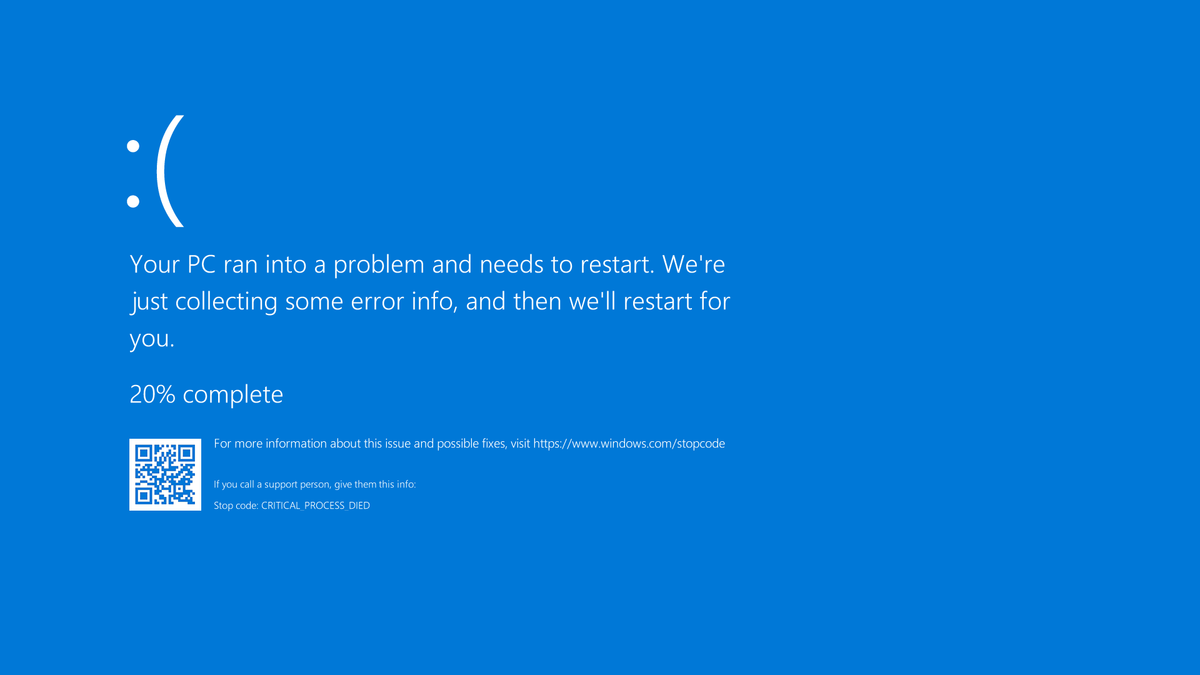
\includegraphics[width=\textwidth]{1.png}
      \end{figure}    
      \vspace*{-5.4cm}
      \textbf{
\huge 全都要背? \hspace*{5pt} !!!}}
\author{NP\_123\\np123greatest@gmail.com}
\date{\today }



\begin{document} 


\maketitle
\tableofcontents
% \addtocontents{toc}{\protect\addvspace{10pt}} % 添加垂直间距
% \addcontentsline{toc}{section}{考试内容}
\addtocontents{toc}{\protect\addvspace{10pt}} % 添加垂直间距
\addcontentsline{toc}{section}{ 考试内容 }


\section*{考试内容}
\begin{enumerate}
    \item 填空题(共20分,每空格 1分)
    \item 选择题(共20分,每小题1分,单选)
    \item 判断题(共10分,每小题1分)
    \item 简答题(15分,每小题3分)
    \item 综合题(35分,每小题7分)
\end{enumerate}
% 标红的标题为复习指导中包括的内容,楷体为预测不考的内容,删除线为没有讲过的内容
\clearpage

\section{操作系统引论}

\subsection{操作系统的目标和作用}
\subsubsection{\color{red}操作系统的目标}
\textbf{什么是操作系统:}
操作系统是控制和管理计算机系统内各种硬件和软件资源、
有效地组织多道程序运行的系统软件(或程序集合),是用户与计算机之间的接口。

\textbf{\sout{操作系统的目标:}}{\color{gray}方便性、有效性、可扩充性、开放性}
\subsubsection{{\color{red}操作系统的作用}}
\noindent 操作系统在计算机系统中处于\textbf{硬件层之上,应用软件层之下}。作用是:
\begin{enumerate}
    \item 用户与计算机硬件系统之间的接口
    \item 计算机系统资源的管理者
    \item 实现了对计算机资源的抽象(扩充机器)
\end{enumerate}

\subsubsection{推动操作系统发展的主要动力}
不断提高计算机资源利用率;方便用户;器件的不断更新换代;
计算机体系结构的不断发展;
不断提出新的应用需求


\subsection{操作系统的发展过程}
\vspace*{-0.3cm}
\subsubsection{\color{gray}未配置操作系统的计算机系统}
\vspace*{-0.3cm}
\subsubsection{\color{gray}单道批处理系统}
\vspace*{-0.3cm}
\subsubsection{\color{red}\sout{(多道)}批处理系统(如结算系统、银行信用卡计费、电视栏目排播等)}
\textbf{发展的主要动力:}提高资源利用率和系统吞吐量

\textbf{定义:}用户作业成批的处理,作业建立、过渡、完成都自动由系统成批完成,
且在计算机内存中同时存放几道相互独立的程序,使它们在管理程序的控制下,相互穿插运行。

\textbf{优点:}资源利用率高、系统吞吐量大。
\textbf{缺点:}平均周转时间长;无交互能力

% {\color{red}多道\textbf{程序设计是在一台计算机上同时运行两个或更多个程序,多道程序设计具有提高系统资源利用率和增加作业吞吐量的优点。}}

\subsubsection{\color{red}分时系统(如UNIX 系统、Linux 系统、Windows 服务器等)}
\textbf{发展的主要动力:}满足用户对人-机交互的需求。

\textbf{定义:}在一台主机上连接了多个配有显示器和键盘的终端并由此组成的系统,
该系统允许多个用户同时通过自己的终端,以交互方式使用计算机,
共享主机中的资源。UNIX是分时操作系统。

\subsubsection{\color{red}实时系统(如工业控制系统、信息查询系统、多媒体系统、嵌入式系统)}
\textbf{定义:}计算机对于外来信息能够以足够快的速度进行处理,
并在被控对象允许的时间范围内做出快速反应。

\subsection{操作系统的基本特性}
\subsubsection{\color{red}并发(Concurrence)}
两个或多个活动在同一给定的时间间隔内进行
\vspace*{-0.4cm}
\subsubsection{\color{red}共享(Sharing)}
计算机系统中的资源被多个任务所共用
\vspace*{-0.4cm}
\subsubsection{\color{red}虚拟(Virtual)}
虚拟处理机、虚拟内存、虚拟外设等
\vspace*{-0.4cm}
\subsubsection{\color{red}异步(Asynchronism)}
多道程序下,各程序的执行过程由程序执行时的现场决定

\subsection{操作系统的主要功能}
\subsubsection{\color{red}处理机管理功能}
进程控制;进程同步;进程通信;调度
\vspace*{-0.4cm}
\subsubsection{\color{red}存储器管理功能}
内存分配、内存保护、内存扩充和地址映射
\vspace*{-0.4cm}
\subsubsection{\color{red}设备管理功能}
缓冲管理、设备分配、设备处理
\vspace*{-0.4cm}
\subsubsection{\color{red}文件管理}
文件存储空间的管理、文件操作的一般管理、目录管理、
文件的读写管理和存取控制、文件的逻辑结构和物理结构。
\vspace*{-0.4cm}
\subsubsection{\color{red}操作系统与用户之间的接口}
书:用户接口、程序接口

复习指导:命令接口、图形接口和系统调用接口

\subsection{\color{red}概念补充}
\begin{itemize}
    \item 分时概念:分时主要指若干并发进程对CPU时间的共享。
    \item 通用操作系统:兼备了批处理、分时和实时操作系统三者或其中二者的功能的操作系统。
    \item 为实现多道程序设计需要有更大的内存
\end{itemize}



\clearpage
\section{进程的描述与控制}
\subsection{前驱图和程序执行(不允许有环)}
\begin{itemize}
    \item 程序顺序执行时的特征:顺序性、封闭性、可再现性
    \item 程序并发执行时的特征:间断性、失去封闭性、不可再现性
\end{itemize}

\subsection{进程的描述}
\subsubsection{{\color{red}进程的定义和特征{\color{green}(背)}}}
\begin{enumerate}
    \item 进程是程序的一次执行。
    \item 进程是一个程序及其数据在处理机上顺序执行时所发生的活动。
    \item 进程是具有独立功能的程序在一个数据集合上运行的过程,它是系统进行资源分配和调度的一个独立单位。
\end{enumerate}
\textbf{进程的特征:}动态性;并发性;独立性;异步性;\textbf{结构特征}。\\
\textbf{进程两个基本属性:}可拥有资源的独立单位、可独立调度和分派的基本单位。\\
\textbf{进程与程序的区别:}

\begin{enumerate}
    \item 程序是静态概念,而进程是程序的一次执行过程,是动态概念。
    \item 进程是一个能独立运行的单位,能与其它进程并发执行。进程是作为申请和调度单位存在的;而通常的程序是不能作为一个独立运行的单位而并发执行的。
    \item 程序和进程无一一对应关系。
    \item 各个进程在并发执行过程中会产生相互制约关系,而程序本身是静态的,不存在这种异步特征。
\end{enumerate}

\subsubsection{{\color{red}进程的基本状态及其变化}}
\noindent\textbf{进程的基本状态:}
\begin{itemize}
    \item 运行态:当前进程已分配到CPU,它的程序正在处理机上运行;
    \item 就绪态:进程已具备运行条件,但因为其它进程正占用CPU,所以暂时不能运行而等待分配CPU的状态;
    \item 阻塞态:因等待某件事件发生而暂时不能运行的状态。
\end{itemize}
\textbf{三种基本状态的转换:}
\begin{itemize}
\item 就绪$\rightarrow$运行:被调度程序选中,分配到CPU。
\item \textbf{运行$\rightarrow$阻塞(only)}:因缺乏某种条件而放弃对CPU的占用。
\item 阻塞$\rightarrow$就绪:阻塞态进程所等待的事件发生了。
\item 运行$\rightarrow$就绪: 进程用完时间片(分时系统中)或一个优先权更高的进程进入就绪队列(“优先权高优先”调度算法中)。
\end{itemize}

\subsubsection{\textcolor{red}{挂起操作和进程状态的转换}}

\begin{wrapfigure}{r}{0.44\textwidth}
    \centering
    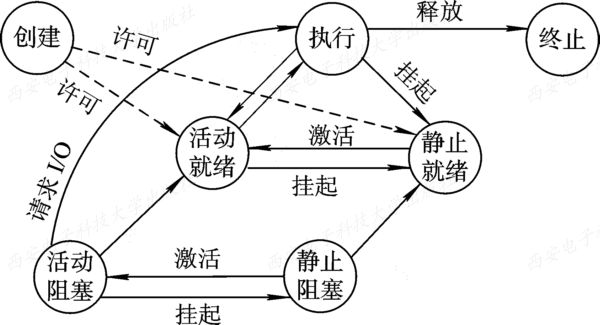
\includegraphics[width=0.44\textwidth,trim=0 20 0 20,clip]{进程状态.png}
\end{wrapfigure}


引入挂起操作的原因,是基于系统和用户的如下需要:

\begin{enumerate}
    \item 终端用户的需要。
    \item 父进程请求。
    \item 负荷调节的需要。
    \item 操作系统的需要。
\end{enumerate}



\subsubsection{{\color{red}进程管理中的数据结构}{\color{green}(背,背,背)}}
\noindent\textbf{PCB的具体作用:{\color{green}(背)}}
\begin{enumerate}
    \item 作为独立运行基本单位的标志\hyperref[进程标识符]{(依据PID)}
    \item 能实现间断性运行方式\hyperref[处理机状态]{(借助处理机状态)}
    \item 提供进程\hyperref[进程调度信息]{调度}所需要的信息:提供了进程处于何种状态的信息\textit{(处于就绪状态调度执行)}
    \item 提供进程\hyperref[进程控制信息]{管理(控制)}所需要的信息:便于OS根据PCB实施对进程的控制和管理
    \item 实现与其它进程的同步与通信
\end{enumerate}
\textbf{重点:PCB中的内容:{\color{green}(背)}}
\begin{enumerate}
    \item \label{进程标识符}进程标识符:外部标识符;内部标识符
    \item \label{处理机状态}处理机状态:由处理机的各种寄存器中的内容组成的
    \begin{enumerate}
        \item 通用寄存器(\textbf{用户可以访问})
        \item 指令计数器
        \item 程序状态字PSW
        \item 用户栈指针
    \end{enumerate}
    \item \label{进程调度信息}进程调度信息
    \begin{enumerate}
        \item 进程状态(就绪?阻塞?)
        \item 进程优先级
        \item 进程调度所需的其它信息(与所采用的进程调度算法有关)
        \item 事件(阻塞原因?)
    \end{enumerate}
    \item \label{进程控制信息}进程控制信息
    \begin{enumerate}
        \item 程序和数据的地址
        \item 进程同步和通信机制
        \item 资源清单
        \item 链接指针(下一个进程的PCB的首地址)
    \end{enumerate}
\end{enumerate}

\subsection{进程控制}
\subsubsection{{\color{red}操作系统内核(处理机的两种执行状态)}{\color{green}(背)}}
系统态:又称为\textbf{管态},也称为内核态。它拥有较高的特权,能执行一切指令,访问所有
寄存器和存储区,传统的OS都在系统态运行。

用户态:又称为\textbf{目态}。它是具有较低特权的执行状态,仅能执行规定的指令,访问指定
的寄存器和存储区。一般情况下,应用程序只能在用户态运行。

{\textbf {\color{red}从目态转换到管态的唯一途径是中断。}}

\subsubsection{进程的创建:}
\noindent\textbf{引起创建进程的事件:{\color{green}(背)}}
\begin{itemize}
    \item 分时系统:典型事件-\textbf{用户登录}
    \item 批处理系统:典型事件-\textbf{作业调度}
    \item 由系统专门为运行中的应用进程创建新进程:\textbf{提供服务}
    \item \textbf{应用请求}
\end{itemize}
\textbf{进程的创建:}
\begin{enumerate}
    \item 申请空白PCB,为新进程申请获得唯一的数字标识符,并从PCB集合中索取一个空白PCB。
    \item 为新进程分配其运行所需的资源,包括各种物理和逻辑资源,如内存、文件、I/O设备和CPU时间等。
    \item 初始化进程控制块(PCB)。
    \item 如果进程就绪队列能够接纳新进程,便将新进程插入就绪队列。
\end{enumerate}
\subsubsection{进程的终止}
\noindent\textbf{引起进程终止的事件:}
\begin{enumerate}
    \item 正常结束
    \item 异常结束:越界错、保护错、非法指令、特权指令错、运行超时、等待超时、
    算数运算错、I/O故障
    \item 外界干预:操作员或操作系统干预、父进程请求、因父进程终止
\end{enumerate}
\textbf{进程的终止过程(太恶心了,待定)}
\subsubsection{进程的阻塞与唤醒(引起进程阻塞(进程主动阻塞)和唤醒的事件)}
\begin{enumerate}
    \item 向系统请求共享资源失败
    \item 等待某种操作的完成
    \item 新数据尚未到达
    \item 等待新任务的到达
\end{enumerate}
\subsection{进程同步}
\subsubsection{{\color{red}进程同步的基本概念}}
\noindent\textbf{两种形式的制约关系{\color{green}(背)}}
\begin{enumerate}
    \item 间接相互制约关系(互斥,Mutex):多个程序在并发执行时,由于共享系统资源,如CPU、I/O设备等,
    致使在这些并发执行的程序之间形成相互制约的关系。
    \item 直接相互制约的关系(同步,Semaphore):进程间的直接制约关系就是源于他们之间的相互合作。
\end{enumerate}
\textbf{什么是临界资源、临界区{\color{green}(背)}}

临界资源:诸进程间采取互斥方式,实现对这种资源的共享;
临界区:人们把在每个进程中访问临界资源的那段代码称为临界区。

\noindent \textbf{进程同步机制应遵循的准则{\color{green}(背)}}

空闲让进、忙则等待、有限等待、让权等待
\vspace*{-0.2cm}
\subsubsection{{\color{red}信号量机制(自求多福)}}
\vspace*{-0.2cm}
\subsubsection{{\color{red}管程}}
定义:进程只能互斥地使用管程,即当一个进程使用管程时,另一个进程必须等待。
当一个进程使用完管程后,它必须释放管程并唤醒等待进入管程的某一个进程。

\vspace*{0.2cm}
\noindent\textbf{四部分组成:{\color{green}(背)}}
\vspace*{-0.2cm}
\begin{enumerate}
    \item 管程的名称
    \item 局部与管程的共享数据结构说明
    \item 对该数据结构进行操作的一组过程
    \item 对局部与管程的共享数据设置初始值的语句
\end{enumerate}

\noindent\textbf{为什么要引入条件变量?{\color{green}(背)}}

当一个进程调用了管程,
在管程中时被阻塞或挂起,直到阻塞或挂起的原因解除,
而在此期间,如果该进程不释放管程,则其它进程无法进入管程,
被迫长时间的等待。
\vspace*{-0.3cm}
\subsection{{\color{gray}典型的进程同步问题}}
\vspace*{-0.2cm}
\subsection{{\color{red}进程通信(待完善)}{\color{green}(背)}}
\begin{enumerate}
    \item 共享存储器系统
    \item 管道通信系统(只适用于父子进程通信)
    \item 消息传递系统(直接通信方式和间接通信方式—信箱)
    \item 客户机-服务器系统
\end{enumerate}

\subsection{线程的基本概念}
\subsubsection{{\color{red}{线程的引入}}{\color{green}(背)}}
\textbf{什么是线程:}线程是进程中能够并发执行的实体,是进程的组成部分,
也是CPU调度和分派的基本单位。允许一个进程中包含一个或多个并发执行的线程,
同一个进程中的所有线程共享其所属进程所拥有的全部资源,
可以为完成某一项任务而协同工作。

上课补充:进程切换需要页表(内外存转化);
线程切换是不需要上下文(共享同一进程的代码段,数据段)

\textbf{为什么引入线程:}是为了减少程序在并发执行时所付出的时空开销。

\textbf{线程的基本状态:}执行状态,就绪状态,阻塞状态
\subsubsection{{\color{red}{进程和线程的比较}}{\color{green}(背)}}
    \begin{enumerate}
        \item \textbf{调度的基本单位:}进程-资源分配和调度;线程-CPU调度和分派
        \item \textbf{并发性:}都可以并发,使得OS具有更好的并发性
        \item \textbf{拥有资源:}进程可以拥有资源;线程本身并不拥有系统资源,但共享所属进程所拥有的资源
        \item \textbf{独立性:}同一进程中的不同线程之间的独立性要比不同进程之间的独立性低得多
        \item \textbf{系统开销:}进程>线程
        \item \textbf{支持多处理机系统:}可以将一个进程中的多个线程分配到多个处理机上,使他们并行执行。
    \end{enumerate}    

\clearpage
\subsection{\color{green}补充:进程同步的例题}
\subsubsection{水果分配}


\begin{tcolorbox}
    [colback=Emerald!10,colframe=cyan!40!black,title=\textbf{伪代码}]
    \begin{lstlisting}[language=C]
    semaphore mutex=1,apple=0,banana=0,empty=20;
    main(){ cobegin{ 
        Process_Father:
        while(true){
            从野外采摘新鲜的水果盲盒;
            P(empty);
            P(mutex);
            putfruit();
            V(mutex);
            if (fruit==apple) V(apple);
            else V(banana);
        }   
        Process_Daughter:
        while(true){
            P(apple);
            P(mutex);
            getapple();
            V(mutex);
            V(empty);
            
            countapple();
        }
        Process_Son:
        while(true){
            P(banana);
            P(mutex);
            getbanana();
            V(mutex);
            V(empty);
            countbanana();
        }
     }coend}\end{lstlisting}
\end{tcolorbox}
\clearpage
\subsubsection{和尚喝水}
某寺庙,有小和尚、老和尚若干。有一水缸,由小和尚用水桶从井中提水入缸,老和尚用水桶从缸里取水饮用。水缸可容10桶水,水取自同一井中。水井径窄,每次只能容一个水桶取水。水桶总数为3个。每次入、取缸水仅为1桶,且不可以同时进行。试用P、V操作给出小和尚、老和尚动作的算法描述。

\begin{tcolorbox}
    [colback=Emerald!10,colframe=cyan!40!black,title=\textbf{伪代码}]
    \begin{lstlisting}[language=c]
    semaphore mutex1=1,mutex2=1,empty=10,full=0,count=3;
    main(){ cobegin{ 
        Process_YoungMonk_i: // i=1,2,... 
        while(true){
            P(empty);
            P(count);
            P(mutex1);
            getWaterFromWell();
            V(mutex1);
            P(mutex2);
            putWaterIntoPot();
            V(mutex2);
            V(count);
            V(full);
        }
        Process_OldMonk_j: // j=1,2,...
        while(true){
            P(full);
            P(count);
            P(mutex2);
            getWaterFromPot();
            V(mutex2);
            V(count);
            V(empty);
        }
    }coend}\end{lstlisting}
\end{tcolorbox}

\clearpage
\subsubsection{生产者消费者}
\begin{tcolorbox}
    [colback=Emerald!10,colframe=cyan!40!black,title=\textbf{伪代码}]
    \begin{lstlisting}[language=c]
    int in=0,out=0;
    Item buffer[n];
    semaphore mutex=1,empty=n,full=0;
    main(){ cobegin{ 
        Process_Produce: 
        while(true){
            Produce an Item in nextp;
            P(empty);
            P(mutex);
            buffer[in]=nextp;
            in=(in+1)%n;
            V(mutex);
            V(full);
        }
        Process_Consume:
        while(true){
            P(full);
            P(mutex);
            nextc=buffer[out];
            out=(out+1)%n
            V(mutex);
            V(empty);
            Consume an Item in nextc;
        }
    }coend}\end{lstlisting}
\end{tcolorbox}

\clearpage
\subsubsection{哲学家问题}
\begin{tcolorbox}
    [colback=Emerald!10,colframe=cyan!40!black,title=\textbf{伪代码}]
    \begin{lstlisting}[language=c]
    semaphore mutex = 1; // For critical section
    semaphore footman = 4; // Max 4 hypocrite eating at the same time
    semaphore forks[5] = {1,1,1,1,1}; // Semaphores for the forks

    main(){ cobegin{ 
        Process_Philosopher(i) {
        while (true) {
            think();
            // Ask permission from the footman
            P(footman);
    
            // Pick up the forks
            P(mutex); // Entering critical section
            P(forks[i]);
            P(forks[(i+1)%5]);
            V(mutex); // Exiting critical section
    
            eat();
    
            // Put down the forks
            P(mutex); // Entering critical section
            V(forks[i]);
            V(forks[(i+1)%5]);
            V(mutex); // Exiting critical section
    
            // Release footman
            V(footman);
        }coend}\end{lstlisting}
\end{tcolorbox}

\clearpage
\subsubsection{读者写者问题}
\begin{tcolorbox}
    [colback=Emerald!10,colframe=cyan!40!black,title=\textbf{伪代码}]
    \begin{lstlisting}[language=C]
    semaphore rmutex = 1, wmutex=1;
    int reader_count = 0;   
    // The number of readers currently accessing the database
    
    procedure Reader {
        while (true) {
            P(rmutex);
            if(reader_count==0) P(wmutex);
            // If this is the first reader, lock(wait for) the writer
            reader_count++; 
            V(rmutex);
            ...
            readDatabase();
            ...
            P(rmutex);
            reader_count--;
            if (reader_count == 0) V(wmutex);  
            // If this is the last reader, unlock the database
            V(rmutex);
        }
    }
    procedure Writer {
        while (true) {
            P(wmutex);
            writeDatabase();
            V(wmutex);
        }
    }\end{lstlisting}
\end{tcolorbox}


\clearpage
\section{处理机调度与死锁}
\subsection{处理机调度的层次和调度算法的目标}
\subsubsection{{\color{red}处理机调度的层次}{\color{green}(背)}}
\begin{enumerate}
    \item 高级调度(长程调度或作业调度)-批处理系统
    
    \textbf{调度对象:作业}
    
    根据某种算法,决定将外存上处于后备队列中的哪几个作业调入内存,为它们创建进程、分配必要的资源,并将它们放入就绪队列。
    \item 低级调度(进程调度或短程调度(频率最高))-三种基本类型
    
    \textbf{调度对象:进程}

    根据某种算法,决定就绪队列中的哪个进程应获得处理机,并由分派程序将处理机分配给被选中的进程。它是最基本的调度。
    \item 中级调度(内存调度)--分时系统
    
    提高内存利用率和系统吞吐量(引入中级调度的原因)。应把那些暂时不能运行的进程,调至外存等待,让他处于挂起状态。

\end{enumerate}

\subsubsection{{\color{red}处理机调度算法的目标}{\color{green}(背)}}
\begin{enumerate}
    \item 处理机调度算法的共同目标
    \begin{enumerate}
        \item 资源利用率
        \[\text{CPU的利用率}=\frac{\text{CPU有效工作时间}}{\text{CPU有效工作时间}+\text{空闲等待时间}}\]
        \item 公平性
        \item 平衡性
        \item 策略强制执行
    \end{enumerate}
    \item 批处理系统的目标(评价调度算法的指标)
    \begin{enumerate}
        \item 平均周转时间短(设作业的周转时间$T_i$)。

        \textbf{周转时间:}是指从作业被提交给系统开始
        到作业完成为止这段时间间隔。
        \vspace*{-0.2cm}
        \begin{equation}
            \begin{split}
                \text{周转时间} =& \text{ 作业在外存后备队列上等待(作业)调度的时间}\\
                    + &\text{ 作业在就绪队列上等待进程调度的时间}\\
                    + &\text{ 进程在 CPU 上执行的时间}\\
                    + &\text{ 进程等待 I/O 操作完成的时间}\nonumber
            \end{split}
            \end{equation}


        \textbf{平均周转时间:}
        \[T=\frac{1}{n}[\sum_{i=1}^nT_i]\]
        \textbf{带权周转时间}(系统为它提供服务时间$T_s$,反映作业对系统资源的使用效率):
        \[W=\frac{T_i}{T_s}\]
        \textbf{平均带权周转时间}(设系统为它提供服务时间$T_s$):
        \[W=\frac{1}{n}\sum_{i=1}^{n}\frac{T_i}{T_s}\]
        \item 系统吞吐量高:\textbf{吞吐量是指单位时间内系统所完成的作业数。}提高吞吐量选择短作业运行
        \item 处理机利用率高:提高处理机利用率选择计算量大的作业运行
    \end{enumerate}
    \item 分时系统的目标:响应时间快,均衡性
    \item 实时系统的目标:截至时间的保证,可预测性
\end{enumerate}

\subsection{作业与作业调度}
\subsubsection{{\color{red}批处理系统中的作业}{\color{green}(背)}}

作业控制块(JCB):包含作业标识、用户名称、用户账号、作业类型
(CPU繁忙型、I/O繁忙型、批量型、终端型)、作业状态、调度信息(优先级、作业运行时间)、
资源需求(预计运行时间、要求内存大小等)、资源使用情况等。

作业运行的阶段:收容阶段-后备状态、运行阶段、完成阶段
\subsubsection{作业调度的主要任务}
接纳多少个作业、接纳哪些作业
\subsubsection{{\color{red}先来先服务(FCFS)和短作业优先(SJF)调度算法}{\color{green}(背)}}
FCFS是最简单的调度算法,该算法\textbf{既可用于作业调度,也可用于进程调度。}
从后备作业队列中选择几个\textbf{最先进入该队列}的作业,将它们调入内存,为它们分配资源和创建进程。然后把它放入就绪队列。
{\color{red}只考虑了作业的等待时间,忽视了作业的运行时间}


短作业优先(SJF)的调度算法,该算法\textbf{既可用于作业调度,也可用于进程调度。}
从外存的作业后备队列中选择若干个\textbf{估计运行时间最短}的作业,优先将它们调入内存运行。
{\color{red}只考虑了作业的运行时间,忽视了作业的等待时间}


缺点:必须与制作业的运行时间;对长作业非常不利;人-机无法实现交互;未考虑作业的紧迫程度
\subsubsection{{\color{red}优先级调度算法(PSA)和高响应比优先调度算法(HRRN)}{\color{green}(背)}}
\label{优先级调度算法}优先级调度算法(PSA):作业优先级有\textbf{静态优先级}(依据:进程类型、进程对资源的需求、用户要求)和\textbf{动态优先级}。
\textit{对于先来先服务调度算法,作业的等待时间就是作业的优先级,
等待时间越长,其优先级越高。对于短作业优先调度算法,作业的长短就是作业的优先级,
作业所需运行的时间越短,其优先级越高。但上述两种优先级都不能反映作业的紧迫程度。}
\vspace*{-0.2cm}
\begin{enumerate}
    \item \hyperref[非抢占式]{非抢占式}优先级调度算法
    \item \hyperref[抢占式]{抢占式}抢占式优先级调度算法:每当出现新的就绪进程$i$时,将其优先级$P_i$
    与正在执行的进程$j$进行比较,如果$P_i \leq P_j$,源进程$P_j$便继续执行;但如果是
    $P_i > P_j$,则立即停止$P_j$的执行,进行进程切换,使$i$进程投入执行。\textbf{常用于对实时性要求较高的系统中。}
\end{enumerate}
\vspace*{1cm}

高响应比优先调度算法(HRRN):
{\color{red}引入动态优先级,不仅考虑了作业的运行时间,还考虑了作业的等待时间}
。优先级,也可以叫响应比$R_P$,可以表示为:
\[\text{优先权}=R_P=\frac{\text{等待时间}+\text{要求服务时间}}{\text{要求服务时间}}=\frac{\text{响应时间}}{\text{要求服务时间}}\]
\begin{enumerate}
    \item 等待时间相同,要求服务的时间愈短,优先权愈高。类似SJF
    \item 要求服务时间相同,等待时间愈高,优先权愈高。类似FCFS
    \item 长作业的优先级会随着等待时间的增加而提高。
\end{enumerate}

\subsection{进程调度}
\subsubsection{进程调度的任务、机制和{\color{red}方式}}
\begin{enumerate}
    \item 进程调度的任务
    \begin{enumerate}
        \item 保存处理机的现场信息:\textit{程序计数器、多个通用寄存器中的内容}
        \item 按某种算法选取进程:\textit{从就绪队列中选取}
        \item 按处理机分配给进程:\textit{将进程控制块内有关处理机现场信息装入处理器相应的各个寄存器中}
    \end{enumerate}
    \item 进程调度机制
    \begin{enumerate}
        \item 排队器:\textit{事先将系统中的所有就绪进程按照一定的策略排成一个或多个队列,以便调度程序能最快地找到他}
        \item 分派器:\textit{依据进程调度程序所选定的进程,将其从就绪队列中取出}
        \item 上下文切换器:\textbf{1.保存当前进程的上下文;2.移出分派程序的上下文,把新选进程的CPU现场信息装入到处理机的各个相应寄存器中,以便新进程运行}
    \end{enumerate}
    \item 进程调度方式{\color{green}(背)}
    \begin{enumerate}
        \item \label{非抢占式}非抢占方式:一旦处理机分配给某进程后,就一直让它运行下去。
        
        \textbf{原因:}正在执行的进程运行完毕或无法运行;提出I/O请求而暂停执行;执行了某种原语操作(如Block)
        \item \label{抢占式}抢占方式:允许调度程序根据某种原则,暂停某个正在执行的进程,将已分配
        该进程的处理机重新分配给另一进程

        \textbf{好处:}批处理机系统:防止一个长进程长时间占用处理机;分时系统:有可能实现人-机无法实现交互
        实时系统:能满足实时任务的需求。

        \textbf{遵循的原则:}优先权原则;短进程优先原则;时间片原则
    \end{enumerate}
\end{enumerate}
\subsubsection{{\color{red}轮转调度算法}{\color{green}(背)}}
隐含的假设:所有的进程急迫性都是相同的,但实际情况并非如此

切换时机:若一个时间片尚未用完,正在运行的进程便已完成,就立即激活调度程序;在一个时间片用完时,计时器中断程序被激活

时间片大小的确定:若时间偏小,则增加系统的开销;若时间片太长,RR算法则退化为FCFS算法。
\subsubsection{\hyperref[优先级调度算法]{优先级调度算法}}
\subsubsection{\sout{多队列调度算法}}
\subsubsection{{\color{red}多级反馈队列调度算法}}
调度机制:{\color{red}(优点:)不必知道各种进程所需的执行时间}
\begin{enumerate}
    \item 设置多个就绪队列,每个队列赋予不同的优先级:优先级愈高的队列时间片愈小
    \item 每个队列都采用FCFS算法:在时间片结束尚未完成则放入下一队列队尾
    \item 按队列优先级调度:首先调度最高优先级队列中的诸进程运行,仅当第一队列空闲时
    才调度第二队列中的进程运行。
\end{enumerate}

调度算法的性能:如果规定第一个队列的时间片略大于多数人机交互所需之处理时间时
,便能较好地满足各种类型用户的需要。
\begin{enumerate}
    \item 终端型用户:只要能使这些作业在第一队列规定的时间片内完成,便可
    使终端型用户感到满意
    \item 短批处理作业用户:对于稍长的作业,也只需要在第二和第三队列各执行一
    时间片完成,其周转时间仍然较短
    \item 长批处理作业用户:它将依次在$1,2,\cdots,n$个位列中运行,然后再按
    轮转方式运行,不必担心作业长期得不到处理
\end{enumerate}

\subsection{\sout{实时调度}}
\subsection{死锁概述}
\subsubsection{{\color{red}资源问题}{\color{green}(背)}}
\begin{enumerate}
    \item 可重用性资源(计算机系统中大多数资源):可供用户重复使用多次,但是每一个可重用性资源中的单元只能分配给一个
    进程使用,不允许多个进程共享。

    每一类可重用性资源中的单元数目是相对固定的,进程在运行期间既不能创建也不能删除。
    \item 可消耗性资源(临时性资源,如进程间通信的信息):
    在进程运行期间,由进程动态地创建和消耗的;
    每一类可消耗性资源在进程运行期间可以不断变化
    \vspace*{0.2cm}
    \hrule    \hrule
    \item 可抢占性资源(CPU和主存):
    某进程在获得这类资源后,该资源可以再被其它进程或系统抢占。
    \item 不可抢占性资源(刻录机、磁带机、打印机):
    一旦系统把某资源分批给该进程后,就不能将它突然收回,只能在进程用完后自行释放。
\end{enumerate}

\subsubsection{{\color{red}计算机系统中的死锁(死锁的起因)}{\color{green}(背)}}
\begin{enumerate}
    \item 竞争不可抢占性资源引起死锁(共享文件时)
    \item 竞争可消耗资源引起死锁(进程之间通信时)
    \item 进程推进顺序不当引起死锁
\end{enumerate}

\subsubsection{{\color{red}死锁的定义、必要条件和处理方法}{\color{green}(背)}}
    \textit{死锁的定义:}在一组进程发生死锁的情况下,
    这组死锁进程中的每一个进程,都在等待另一个死锁进程所占有的资源。

    \textbf{产生死锁的必要条件:}{\color{red}互斥条件(无法破坏);请求和保持条件;不可抢占条件;循环等待条件}

    处理死锁的方法(与具体方法相对应):
    \begin{enumerate}
        \item 预防死锁:资源有序分配法
        \item 避免死锁:银行家算法
        \item 检测死锁:资源分配图化简法
        \item 解除死锁:
    \end{enumerate}


\subsection{预防死锁}
\subsubsection{{\color{red}破坏“请求和保持”条件}{\color{green}(背)}}
\textbf{第一种协议:}所有进程开始运行之前,必须一次性地申请其在整个运行过程中
所需的全部资源。

\textbf{优点:}简单、易行且安全。

\textbf{缺点:}资源被严重浪费,进程经常会发生饥饿现象。

\vspace{0.4cm}

\textbf{第二种协议:}允许一个进程只获得运行初期所需的资源后,便开始运行。
进程运行过程中再逐步释放已分配给自己的、且已用完毕的全部资源。

\subsubsection{{\color{red}破坏“不可抢占”条件}{\color{green}(背)}}
当一个已经保持了某些不可抢占资源的进程,提出新的资源请求而不能得到满足时,
它必须释放已经保持的所有资源,待以后需要时再重新申请。

\textbf{缺点:}实现起来比较复杂,需付出很大的代价。
\subsubsection{{\color{red}破坏“循环等待”条件}{\color{green}(背)}}
对系统所有资源类型进行线性排序,并赋予不同的序号。
规定每个进程必须按序号递增的顺序请求资源。
\textbf{与前两种策略相比,资源利用率和系统吞吐量都有较明显的改善}

\textbf{缺点:}限制了新类型设备的增加;作业使用各类资源的顺序与系统规定的顺序不同,
造成对资源的浪费;限制用户简单、自主地编程。

\subsection{避免死锁}
\subsubsection{{\color{red}系统安全状态}}
\textbf{安全状态:}系统能按某种进程推进顺序$(P_1,P_2,\cdots,P_n)$为每个进程
$P_i$分配其所需资源,直至满足每个进程对资源的最大需求,使每个进程都可顺利地完成。

\textbf{安全序列:}此时的$(P_1,P_2,\cdots,P_n)$。

\textbf{不安全状态:}系统无法找到这样的一个安全序列。如果不按照安全序列
分配资源,则系统可能会由安全状态进入不安全状态。

\subsection{{\color{gray}利用银行家算法避免死锁(实验)}}
\subsection{死锁的检测与解除}
\subsubsection{{\color{red}死锁的检测}{\color{green}(背)}}
利用\textbf{资源分配图}检测死锁:$S$为死锁状态的充分条件是:当且仅当$S$状态的资源分配图是不可完全简化的。
该充分条件被成为\textbf{死锁定理}。
\subsubsection{{\color{red}死锁的解除}{\color{green}(背)}}
抢占资源:从一个或多个进程中抢占足够数量的资源,分配给死锁进程,以解除死锁状态。

终止(撤销)进程:终止所有死锁进程;逐个终止进程



\clearpage
\section{存储器管理}
\subsection{\sout{存储器的层次结构}\color{red}(存储器的基本概念)}
存储器管理的功能:内存分配、地址映射、内存保护、内存扩充。

内存以字节为单位进行编址,CPU按内存中的地址读出内存中的内容。
\subsection{程序的装入和链接}
用户程序的主要处理阶段:编辑、\textbf{编译、链接(三种方式)、装入(三种方式)}、运行
\subsubsection{\color{red}程序的装入}
\begin{enumerate}
    \item 绝对装入方式:用户程序经编译后,将产生绝对地址(物理地址)的目标代码
    \item 可重定位装入方式
    
    \textbf{重定位:}在装入时对目标程序中指令和数据地址的修改过程

    \textbf{静态重定位:}地址变换通常是在进程装入时一次完成的,以后不再改变

    \item 动态运行时的装入方式(\label{动态重定位}\textbf{动态重定位}):把装入模块装入内存后,并不立即把装入模块中的
    逻辑地址转换为物理地址,而是把这种地址转换推迟到程序真正要执行时才进行。
    
    \textbf{这种方式需要一个重定位寄存器的支持:}真正访问的内存地址
    是相对地址与重定位寄存器中的地址相加而形成的。
\end{enumerate}

\subsubsection{\color{red}程序的链接}
\begin{enumerate}
    \item 静态链接方式-需要解决的问题:对相对地址进行修改;变换外部调用符号
    \item 装入时动态链接(边装入边链接)-在装入一个目标模块时,若发生一个外部
    模块调用事件,将引起装入程序去找出相应的外部目标模块。
    
    优点:便于修改和更新;便于实现对目标模块的共享
    \item 运行时动态链接-对某些模块的链接推迟到程序执行时才进行。
\end{enumerate}

\subsection{\color{red}连续分配存储管理方式 }
\subsubsection{\color{red}单一连续分配}
整个内存的用户空间由一道用户程序独占。
\vspace*{-0.4cm}
\subsubsection{\color{red}固定分区分配(产生内碎片)}
\begin{enumerate}
    \item 划分分区的方法:分区大小相等;分区大小不等
    \item 内存分配:将分区按其大小进行排队,并为之建立一张分区使用表(起始地址、大小及状态)。
    当有一用户程序要装入时,由内存分配程序依据用户程序的大小检索该表。
\end{enumerate}

\subsubsection{\color{red}动态分区分配(产生外碎片)}
\begin{enumerate}
    \item 动态分区分配中的数据结构:空闲分区表;空闲分区链
    \item 动态分区分配算法
    
    顺序搜索:首次适应、循环首次适应、最佳适应、最坏适应

    索引搜索:快速适应、伙伴系统
    \item 分区分配操作:分配内存、回收内存
    
    \textbf{内存回收时的四种情况}
    \begin{enumerate}
        \item 回收区与插入点的前一个空闲分区$F_1$相邻接,与前一分区合并。\textit{只修改前一分区$F_1$的大小}
        \item 回收区与插入点的后一个空闲分区$F_2$相邻接,与后一分区合并。\textit{用回收区的首址作为新空闲区的首址,大小为两者之和}
        \item 回收区同时与插入点的前、后两个分区相邻接,将三个分区合并。\textit{使用$F_1$的表项和$F_1$的首址,取消$F_2$的表项,大小为三者之和}
        \item 回收区既不与$F_1$相邻接,也不与$F_2$相邻接。\textit{为回收区单独创立一个新表项,填写回收区的首址和大小}
    \end{enumerate}
\end{enumerate}

\subsubsection{\color{red}基于顺序搜索的动态分区分配算法}
\begin{enumerate}
    \item 首次适应(FF)算法:从链首开始顺序查找,直到找到一个大小能满足要求的空闲分区为止
    \item 循环首次适应(NF)算法:不再从链首开始查找,而是从上次找到的空闲分区的下一个空闲分区开始查找
    \item 最佳适应(BF)算法:总能把满足要求、又是最小的空闲分区分配给作业
    \item 最坏适应(WF)算法:总是挑选一个最大的空闲区,分割一部分存储空间给作业使用。
    
    \textbf{好处:}产生碎片的可能性最小,对中、小作业有利。
\end{enumerate}
\vspace*{-0.4cm}
\subsubsection{基于索引搜索的动态分区分配算法}
 快速适应算法;伙伴系统;哈希算法
\vspace*{-0.4cm}
\subsubsection{\color{red}动态可重定位分区分配}
\begin{enumerate}
    \item 利用紧凑(移动)技术把内存中的作业分区链接
    到一起,使分散的空闲区合并成一个大的空闲区。
    \item \hyperref[动态重定位]{动态重定位:}
    
    补充:当系统对内存进行了“紧凑”,而使若干程序从内存的
    某一处移至另一处时,不需对程序做任何修改,只要用该程序在内存的新起始地址
    去置换原来的起始地址即可
    \item 动态重定位分区分配算法:当找不到一个足够大的空闲分区以
    满足用户需求时,如果所有的小的空闲分区的容量总和大于用户的要求,
    这时便须对内存进行“紧凑”,将经“紧凑”后所得到的空闲分区分配给用户。
\end{enumerate}
\vspace*{-0.8cm}
\subsection{\sout{对换}}
\clearpage
\subsection{分页存储管理方式}
\subsubsection{分页存储管理的基本方法}
页号为P,逻辑地址空间中的地址为A,页面的大小为L,偏移量为W,即页内地址

\[\text{P}=\text{INT}[\frac{\text{A}}{\text{L}}],\hspace*{5pt} \text{d}=[\text{A}]\hspace*{1pt}\text{MOD}\hspace*{1pt}\text{L}\]

常在页表的表项中设置一存取控制字段,用于对该存储块中的内容加以保护。
\subsubsection{\color{red}地址变换机构}
\begin{figure}[h]
    \centering
    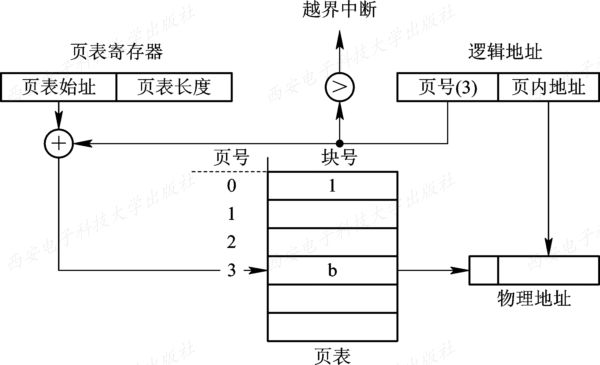
\includegraphics[width=0.4\textwidth]{地址变换.png}
    \hspace*{15pt}
    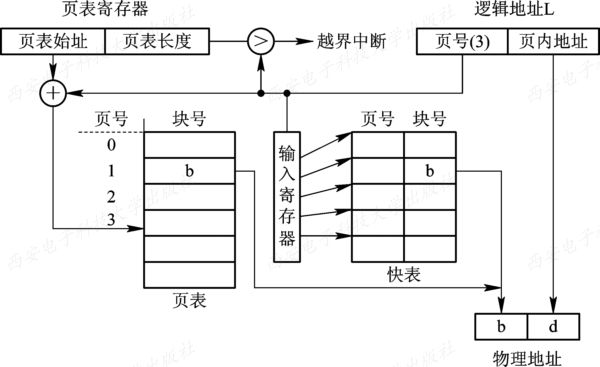
\includegraphics[width=0.4\textwidth]{块表地址变换.png}
\end{figure}   
\subsubsection{\color{red}访问内存的有效时间}
假设访问一次内存的时间为$t$,$a$表示命中率,$\lambda$表示查找块表所需要的时间
\[\text{EAT}=a\times\lambda+(1-a)(t+\lambda)+t=2t+\lambda-t\times a \]

\subsubsection{\color{red}两级和多级页表}
虽然解决了对于大页表无需大片连续储存空间的问题,
但并未解决用较少的内存空间去存放大页表的问题。

用较少的内存空间存放页表的唯一方法是,仅把当前
需要的一批页表项调入内存,以后再根据需要陆续调入。
为了表征某页的页表是否已经调入内存,还应在外层页表项
中增设一个状态为S,表示分页是否在内存中

\subsection{分段存储管理方式}
\subsubsection{分段存储管理方式的引入}
方便编程;信息共享;信息保护;动态增长;动态链接

\subsubsection{\color{red}分段系统的基本原理(访问两次内存)}
分页和分段的主要区别:
\begin{enumerate}
    \item 页是信息的物理单位;分段存储管理方式中的段则是信息的逻辑单位
    \item 页的大小固定且由系统决定;段的长度却不固定,决定于用户所编写的程序
    \item 分页的用户程序地址空间是一维的;分段系统中既需要给出段名,又需给出段内地址
\end{enumerate}
\begin{figure}[h]
    \centering
    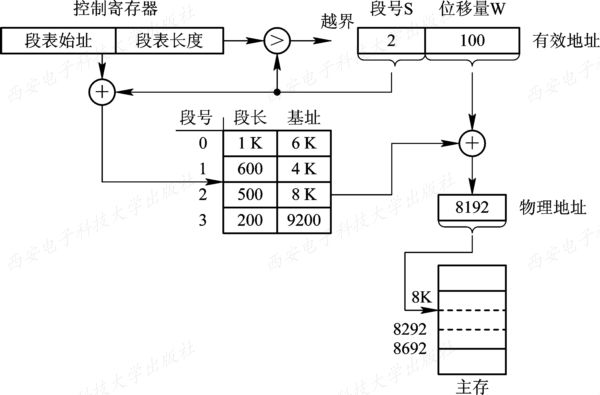
\includegraphics[width=0.6\textwidth]{分段.png}
\end{figure}   

\subsubsection{\color{red}信息共享}
可重入代码(纯代码)是一种允许多个进程同时访问的代码,绝对不允许
可重入代码在执行中有任何改变。   

\subsubsection{\color{red}段页式存储管理方式(访问三次内存)}
\vspace*{-0.7cm}
\begin{figure}[h]
    \centering
    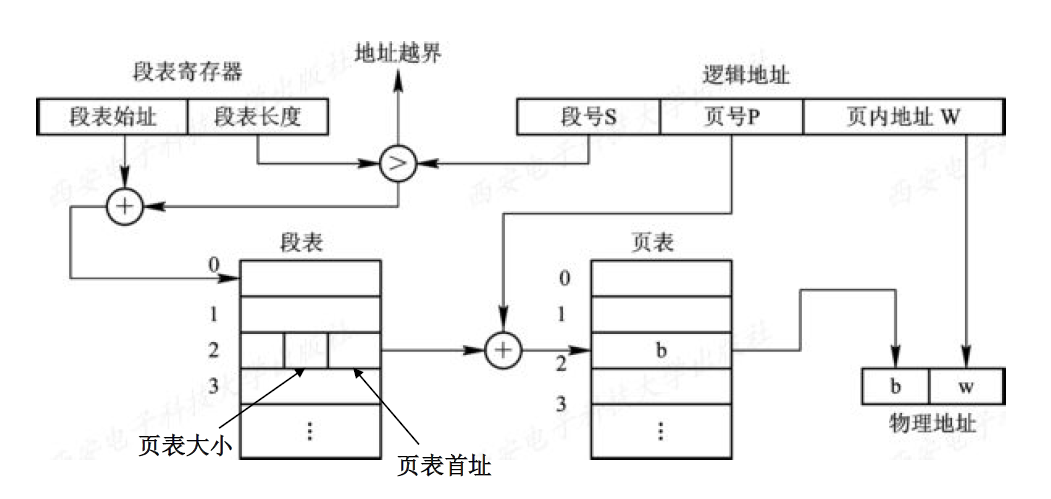
\includegraphics[width=0.8\textwidth]{段页式.png}
\end{figure} 

\clearpage
\section{虚拟存储器}
\subsection{虚拟存储器概述}
\subsubsection{\sout{常规存储管理方式的特征和局部性原理}}
局部性表现在:时间局部性(for)、空间局部性(array)
\subsubsection{\color{red}虚拟存储器的定义和特征}
\begin{enumerate}
    \item \textbf{虚拟存储器的定义:}具有请求调入功能和置换功能,
    能从逻辑上对内存容量加以扩充的一种存储器系统。其逻辑容量由内存容量
    和外存容量之和所决定,其运行速度接近于内存速度,而每位的成本却又接近于外存。
    \item \textbf{虚拟存储器的特征:}多次性;对换性;虚拟性(以多次性和对换性为基础)
\end{enumerate}

\subsubsection{虚拟存储器的实现方法}
\textbf{分页请求系统}-硬件支持:请求分页的页表机制,缺页中断机构,地址变换机构

\textbf{请求分段系统}-硬件支持:请求分段的段表机制,缺段中断机构,地址变换机构

{\color{green}虚拟存储器可管理的空间直接取决于处理器中地址寄存器的位数。}

\subsection{请求分页存储管理方式}
\subsubsection{\color{red}请求分页中的硬件支持}
\begin{enumerate}
    \item 请求页表机制
    
\begin{enumerate}
    \item 状态位(存在位):1bit,指示该位是否已调入内存
    \item 访问字段A:用于记录本页在一段时间内被访问的次数,
    或记录本页最近已有多长时间未被访问,提供给置换算法在选择换出页面时参考
    \item 修改位M:标识该页在调入内存后是否被修改过
    \item 外存地址:指出该页在外村上的地址
\end{enumerate}
\vspace*{-0.8cm}
\begin{center}
    \begin{tabular}{|c|c|c|c|c|c|}
        \hline
        {\color{gray}页号}{\color{red}(n)} & {\color{gray}物理块号}{\color{red}(n)} 
        & 状态位(存在位){\color{red}(1-bit)} & 访问字段A{\color{red}(n)} 
        & 修改位M{\color{red}(1-bit)} & 外存地址{\color{red}(address)} \\
        \hline
    \end{tabular}
\end{center}
    \item 缺页中断机构:在指令执行期间产生和处理中断信号;一条指令在
    执行期间可能产生多次缺页中断。
    \item 地址变换机构(请求分页中的地址变换过程)
    \clearpage
    \begin{figure}[h]
        \centering
        % \vspace*{-2cm}
        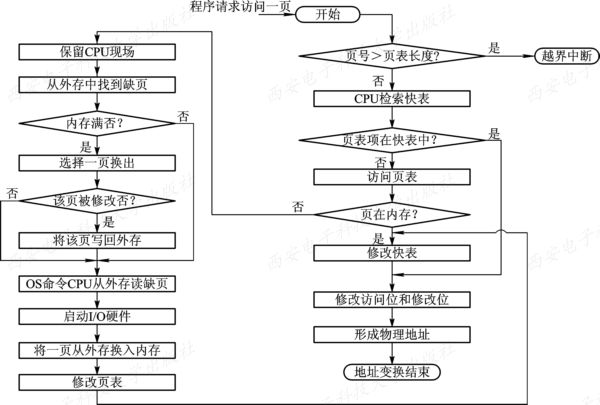
\includegraphics[width=0.6\textwidth]{请求分页地址变化.png}
    \end{figure} 
\end{enumerate}

\subsubsection{请求分页中的内存分配}
\begin{enumerate}
    \item 最小物理块数:小于它,进程不能正常运行
    \item 内存分配策略:
    \begin{enumerate}
        \item 固定分配局部置换:为每个进程分配一定数目的物理块,在整个运行期间都不改变。若进程在运行中发生缺页,则只能从该进程在内存中的页面中选出一页换出,然后再调入需要的页面。
        \item 可变分配全局置换:为系统中的每个进程分配一定数目的物理块,操作系统自身也保持一个空闲物理块队列。当某进程发生缺页时,系统从空闲物理块队列中取出一个物理块分配给该进程,并将欲调入的页装入其中。
        \item 可变分配局部置换:为每个进程分配一定数目的物理块,当某进程发生缺页时,只允许从该进程在内存的页面中选出一页换出,这样就不会影响其他进程的运行。如果进程在运行中频繁地缺页,系统再分配若干物理块给该进程,直至该进程缺页率趋于适当程度;反之,若进程在运行中缺页率特别低,则可适当减少分配给该进程的物理块。
    \end{enumerate}
    \item 物理块分配算法:平均分配算法;按比例分配算法;考虑优先权的分配算法。
\end{enumerate}

\subsubsection{页面调入策略}
\begin{enumerate}
    \item 何时调入页面
    \begin{enumerate}
        \item 预调页策略:将那些预计在不久之后便会被访问的页面预先调入内存
        \item 请求调页策略:若发现其所在的页面不在内存,便立即提出请求。
    \end{enumerate}
    \item 从何处调入页面:系统拥有/缺少足够的对换区空间,UNIX方式
    \item 页面调入过程:保留CPU环境,分析中断原因后转入缺页中断处理程序。
    \item 缺页率:访问页面失败的次数为$F$,总的页面访问次数为$A$,缺页率为
    \[f=\frac{F}{A}\]
\end{enumerate}

\subsection{页面置换算法}
\subsubsection{\color{red}最佳置换算法和先进先出置换算法}
\textbf{最佳置换算法:}保证获得最低的缺页率,是无法实现的。用来评价其它算法

\textbf{先进先出置换算法:}总是淘汰最先进入内存的页面,但与进程实际运行的规律不相适应

\textbf{先进先出算法的Belady异常现象:}在某些情况下,如果内存容量增大了反而会导致缺页次数变多的现象。


\subsubsection{\color{red}最近最久未使用和最少使用置换算法}
\textbf{LRU置换算法:}选择现有页面中t值最大的,即最近最久未使用的页面淘汰(寄存器或栈)

\textbf{最少使用置换算法:}最近时期使用最少的页面作为淘汰页。(移位寄存器)

\subsubsection{\color{red}Clock(最近未用)置换算法}
\noindent 改进型Clock置换算法的四种类型的页面:
\begin{itemize}
    \item 1类(A=0,M=0):最近既未被访问,又未被修改,是最佳淘汰页
    \item 2类(A=0,M=1):最近被访问,但已被修改,并不是很好的淘汰页
    \item 3类(A=1,M=0):最近已被访问,未被修改,有可能再被访问
    \item 4类(A=1,M=1):最近已被访问,又以被修改,有可能再被访问
\end{itemize}
算法的执行过程
\begin{enumerate}
    \item 第一次扫描寻找A=0,M=0的页;
    \item 若失败进行第二次扫描,寻找A=0,M=1的页,同时把遇到的A为1的都改为0;
    \item 若仍失败,重复(1),寻找A=0,M=0的页面;若仍失败,则重复(2),此时一定能找到淘汰页。
\end{enumerate}

\textbf{优点:}替换时首选没有变化的页。由于修改过的页在被替换之前必须写回,因而这样做会节省时间。
\subsubsection{\sout{页面缓冲算法}}
\vspace*{-0.2cm}
\subsection{\sout{“抖动”与工作集}}
\vspace*{-0.2cm}

\subsection{请求分段存储管理方式}
\subsubsection{\color{red}请求分段中的硬件支持}
\begin{enumerate}
    \item 请求段表机制
    \begin{enumerate}
        \item 存取方式:只执行、只读和允许读/写
        \item 增补位:本段在运行过程中是否做过动态增长
    \end{enumerate}

    \begin{center}
        \begin{adjustbox}{width=\textwidth,center}
            \begin{tabular}{|c|c|c|c|c|c|c|c|c|}
                \hline
                {\color{gray}段名} & {\color{gray}段长}& {\color{gray}段基址}
                & 存取方式{\color{red}(2-bit)} & 访问字段A
                & 修改位M & 存在位P
                & 增补位   & 外存地址{\color{red}(address)} \\
                \hline
            \end{tabular}
        \end{adjustbox}
    \end{center}
    \item 缺段中断机构
    \item 地址变换机构
\end{enumerate}




\end{document}